\documentclass[9pt,fleqn,twoside,twocolumn]{stdglobal}

\fancypagestyle{titlepagestyle}{
  \fancyhf{}
  \fancyhead[L]{\footnotesize\itshape Seminar (Illustrative Visualization) 2021/2022}
  % \fancyfoot[C]{\footnotesize\bigskip\thepage/\pageref{LastPage}}
  % \fancyfoot{}
  \fancyfoot[C]{\footnotesize\bigskip\thepage}
  \fancyfoot[RO]{\footnotesize\bigskip\copyright\ Markus Pawellek, \today}
  \renewcommand{\footrulewidth}{0.5pt}
  \renewcommand{\headrulewidth}{0pt}
}

\fancypagestyle{mystyle}{
  \fancyhf{}
  \fancyfoot[C]{\footnotesize\bigskip\thepage}
  \fancyfoot[RO]{\footnotesize\bigskip\copyright\ Markus Pawellek, \today}
  % \fancyhead[LO,RE]{\footnotesize \thetitle} %left
  % \fancyhead[RO,LE]{\footnotesize \theauthor} %right
  % \fancyhead[LO,RE]{\footnotesize \ \smallskip}
  \fancyhead[LE]{\footnotesize\itshape Photic Extremum Lines \smallskip} %right
  \fancyhead[RO]{\footnotesize\itshape Seminar (Illustrative Visualization) 2021/2022\smallskip } %right
  \renewcommand{\headrulewidth}{0.5pt}
  \renewcommand{\footrulewidth}{0.5pt}
}

\usepackage{titlesec}
\titleformat{\section}{\normalfont\bfseries}{\thesection}{1em}{}
\titleformat{\subsection}{\normalfont\small\bfseries}{\thesubsection}{1em}{}

\title{Photic Extremum Lines}
\author{Markus Pawellek}
\date{\today}

\hypersetup{
  pdftex,
  % pdfauthor={Your Name},
  % pdftitle={The Title},
  % pdfsubject={\@title},
  pdfkeywords={Illustrative Visualization; Non-Photorealistic Rendering; Feature Lines; Object-Space Algorithm; Contours; Silhouettes; Suggestive Contours; Photic Extremum Lines; Illumination},
  % pdfproducer={Latex with hyperref},
  % pdfcreator={pdflatex, or other tool}
}

\bibliography{references}

\pagestyle{mystyle}

\begin{document}

\selectlanguage{english}

\thispagestyle{titlepagestyle}

\twocolumn[{\begin{@twocolumnfalse}%
  \begin{center}
    \Large
    \bfseries
    Photic Extremum Lines
  \end{center}%
  %\hfill\rule{0.5\textwidth}{0.5pt}\hfill
  \vspace{1pt}
  \begin{center}
    Markus Pawellek \\
    markus.pawellek@mailbox.org
  \end{center}
  \vspace{1em}
  \begin{center}
    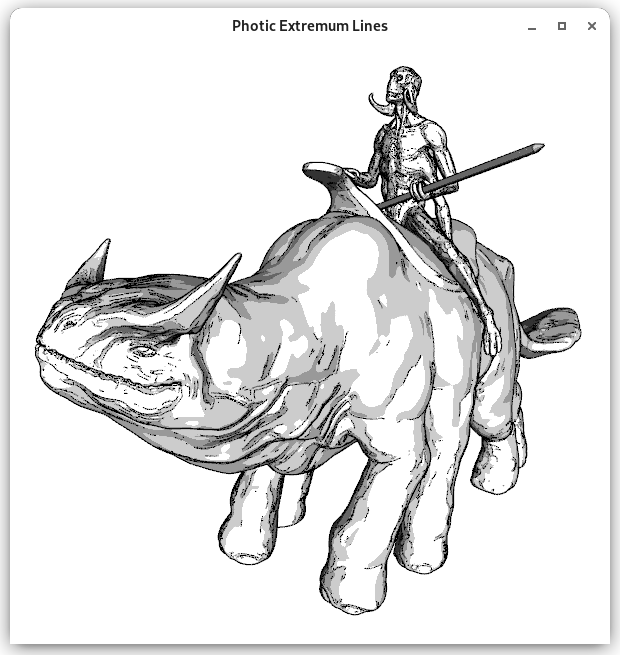
\includegraphics[width=0.24\textwidth,trim={15px 15 15 50},clip]{images/rider.png}
    \hfill
    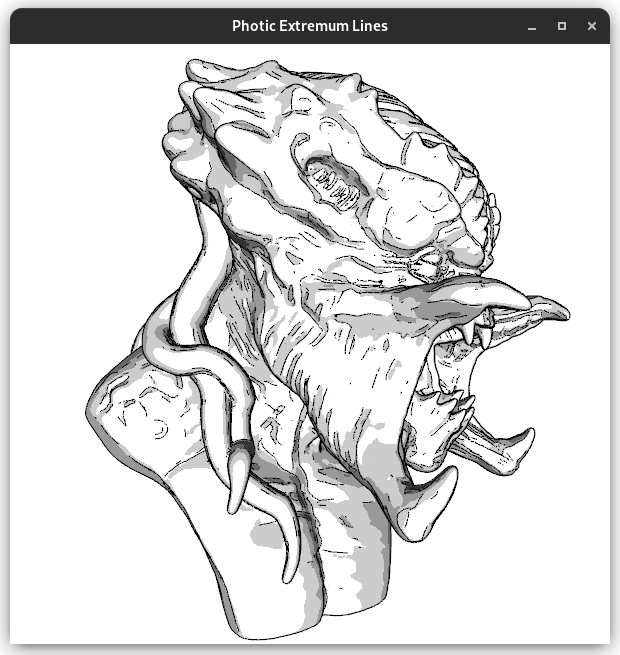
\includegraphics[width=0.24\textwidth,trim={15px 15 15 50},clip]{images/predator-intro.png}
    \hfill
    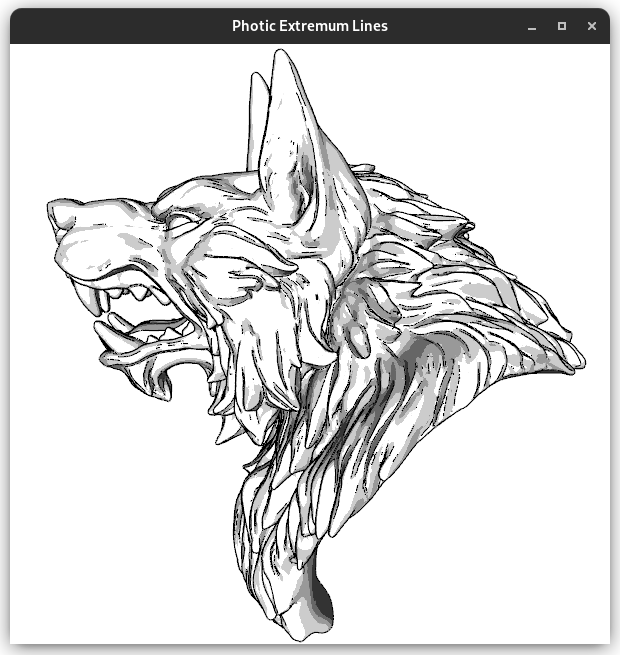
\includegraphics[width=0.24\textwidth,trim={15px 15 15 50},clip]{images/werewolf-intro.png}
    \hfill
    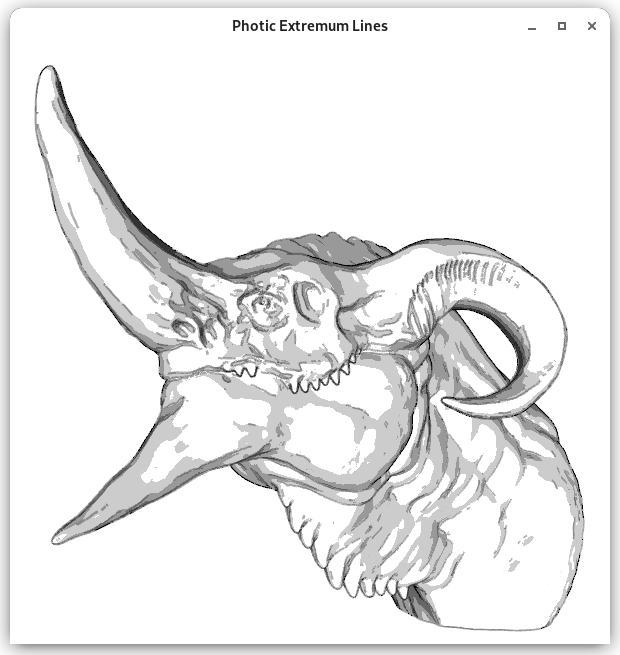
\includegraphics[width=0.24\textwidth,trim={15px 15 15 50},clip]{images/dragon-head-contour-pel-toon-shader.png}
  \end{center}
  \vspace{2em}
  \hrule
  \begin{abstract}
    \itshape
    \noindent
    In the field of illustrative visualization, feature lines are essential for conveying the shape of a given object.
    Photic extremum lines (PELs) are a type of feature lines in object space, which are, besides surface geometry and view position, dependent on the illumination.
    In this way, illustrations generated by PELs strongly coincide with line drawings created by hand due to human perception.
    Furthermore, PELs are easily adjustable by switching between lighting models and allow various post-processing techniques for line stylization and shading.
    The algorithm to extract PELs from scenes mainly has to compute up to third-order derivatives for each vertex and may be parallelized.
    Implementations allowing real-time performance exist for the CPU and GPU.
    By comparison to other feature line types, it can be seen that PELs are an effective and flexible tool for scientific illustration.
    \\

    \noindent
    \textbf{Keywords:}
    \parbox[t]{0.8\textwidth}{Illustrative Visualization, Non-Photorealistic Rendering, Feature Lines, Object-Space Algorithm, Contours, Silhouettes, Suggestive Contours, Photic Extremum Lines, Illumination}
  \end{abstract}
  \hrule
  \vspace{3em}
\end{@twocolumnfalse}}]

\section{Introduction}
  Illustrative visualization is the science and art of effectively communicating known aspects of scientific data in an accurate and intuitive way.
  Especially for the rendering of volumetric data sets in medicine, it is a valuable tool to reduce a vast amount of complex information to its essence.
  In this respect, photorealistic rendering techniques are suboptimal because they are not able to efficiently depict features of interest.
  Our knowledge of human cognition shows that, artistic drawings or paintings, in comparison to a photograph of the same scene, seem to be more suitable for communication and more pleasing in visual experience \autocite{xie2007}.
  Therefore non-photorealistic rendering techniques, typically inspired by artistic styles, are used to create such illustrations.
  \autocite{viola2005}%
  \footnote{In this report, citations concerning more than one sentence are given at the end of the respective paragraph.}

  Feature lines represent a given data set as a line drawing to mimic hand-drawn illustrations.
  In such a way, a large amount of information can be communicated in a succinct manner by taking advantage of human visual acuity.
  Used as an abstraction tool in illustrative visualization, feature lines convey the shape of objects much more efficiently compared to a photograph.
  \autocite{xie2007,isenberg2003,viola2005}

  There are many different types of commonly-used feature lines, such as contours \autocite{isenberg2003}, suggestive contours \autocite{decarlo2003}, ridge-valley lines \autocite{ohtake2004}, apparent ridges \autocite{judd2007}, and demarcating curves \autocite{kolomenkin2008}.
  Typically, these only depend on the surface geometry, such as normal and curvature, and possibly the view position.
  However, human perception is highly sensitive to high variations in illumination.
  As a consequence, for conveying the shape of objects according to human perception, feature lines should also depend on the lighting of an object.
  \autocite{xie2007,zhang2011}

  In this report, we present the concept and implementation of photic extremum lines (PELs), one of the first types of feature lines exhibiting a dependency on illumination.
  PELs have been first introduced in \textcite{xie2007} and further developed in \textcite{zhang2010}.
  Strongly inspired by the edge detection techniques for 2D images, they are characterized by a sudden change of illumination on the surface of a 3D object.
  Since their computation is taken out in object space, PELs are flexible and enable further post-processing such as line stylization and shading \autocite{isenberg2003}.
  Furthermore, by manipulating the illumination of an object, the user can take full control to adjust the rendering output and achieve desired illustration results.
  Implementations for PELs can be done for the CPU and GPU, nowadays, achieving real-time performance.
  \autocite{xie2007,zhang2010}

\section{Related Work}
\label{sec:related-work}

  For the comprehension and implementation of PELs, we also need to rely on several basic techniques and definitions.
  In \textcite{isenberg2003}, we get a thorough classification of feature line types together with recommendations according to the requirements of an application.
  It also describes the general routine for feature line extraction by using subpolygon interpolation which is also used in \textcite{zhang2010} to render PELs.
  Furthermore, a basic but general approach for the hidden line removal for object-space algorithms by using a two-pass rendering with depth buffer testing is provided.
  And additionally, using the above techniques the algorithm for extracting the contours of an object is explained.
  \autocite{isenberg2003}

  The definition of PELs involves up to third-order derivatives of scalar illumination functions given on a triangle mesh.
  Algorithms to correctly estimate curvatures and such derivatives are given in \textcite{rusinkiewicz2004}.
  The main content of this report is based on \textcite{xie2007} which defines PELs and provides a first algorithm and a whole framework to properly generate them.
  Supposable, the algorithm was implemented using the CPU.
  In \textcite{zhang2010}, an improved real-time implementation for PELs on the GPU using the standard graphics pipeline for gradient computations is described.
  Hereby, the authors have used a simpler threshold test and a transformed equation to estimate derivatives for vertices.

  % At this time not used.
  % Use it in conclusions.
  % \autocite{kindlmann2003}
  % \autocite{rusinkiewicz2006}
  % \autocite{kolomenkin2008}

\section{Mathematical Preliminaries}
  To systematically comprehend the definition, design, and implementation of PELs, basic knowledge in differential geometry is administrable.
  In the following, we will repeat the definitions and formulas for gradients and directional derivatives of functions defined on a two-dimensional surface.

  For this section, let $S$ be smooth two-dimensional surface patch and $x\in S$ be an arbitrary point.
  We assume $u,v\in\mathrm{T}_x(S)\subset\setReal^3$ to be vectors that span the tangent space of $S$ at the point $x$.
  Furthermore, let $\function{f,g}{S}{\setReal}$ be two continuously differentiable scalar functions on $S$.
  To be able to express the gradient of such functions, we need the first fundamental form.

  \begin{definition*}[(First Fundamental Form)]
    The first fundamental form $\mathrm{I}_{uv}(x)$ of $S$ at $x$ in $uv$-coordinate representation is given by
    \[
      \mathrm{I}_{uv}(x) \define
      \begin{pmatrix}
        \norm{u}^2 & \scalarProduct{u}{v} \\
        \scalarProduct{u}{v} & \norm{v}^2
      \end{pmatrix} \ .
    \]
    As direct result, its inverse can be computed in the following way.
    \[
      \mathrm{I}^{-1}_{uv}(x) = \frac{\adj \mathrm{I}_{uv}(x)}{\det \mathrm{I}_{uv}(x)}
    \]
    \[
      \adj\mathrm{I}_{uv}(x) =
      \begin{pmatrix}
        \norm{v}^2 & -\scalarProduct{u}{v} \\
        -\scalarProduct{u}{v} & \norm{u}^2
      \end{pmatrix}
    \]
    \[
      \det\mathrm{I}_{uv}(x) = \norm{u}^2\norm{v}^2 - \absolute{\scalarProduct{u}{v}}^2
    \]
  \end{definition*}

  \noindent
  By using $[r]_{uv} = \mathrm{I}_{uv}(x)\, r$, these expressions allow us to freely transform the $uv$-coordinate representation $[r]_{uv}\in\setReal^2$ of tangent space vectors $r\in\mathrm{T}_x(S)$ back and forth to their standard representation.

  \begin{definition*}[(Directional Derivative)]
    Let $w\in\mathrm{T}_x(S)$ be an arbitrary direction.
    Then the directional derivative $\partial_w f(x)$ of $f$ at point $x$ in direction $w$ is given as follows.
    \[
      \partial_w f(x) = \scalarProduct{\nabla f(x)}{w}
    \]
  \end{definition*}

  \noindent
  This definition was provided for the sake of completion.
  Using the definition of directional derivatives together with the expressions based on the first fundamental form, the computation of the gradient of a given scalar function on the surface is then straightforward.

  \begin{definition*}[(Gradient)]
    Let $[\nabla f(x)]_{uv}$ be the $uv$-coordinate representation of $\nabla f(x)$.
    Then the following holds.
    \begin{align*}
      [\nabla f(x)]_{uv} &= \mathrm{I}^{-1}_{uv}(x)
      \begin{pmatrix}
        \partial_u f(x) \\
        \partial_v f(x)
      \end{pmatrix} \\
      \nabla f(x) &=
      \begin{pmatrix}
        u & v
      \end{pmatrix}
      [\nabla f(x)]_{uv}
    \end{align*}
  \end{definition*}

  \noindent
  The definition of PELs involves a more complicated derivative operator to precisely formulate the requirements for a local maximum in a specific direction.

  \begin{definition*}[(PEL Operator)]
    The PEL operator defined as follows evaluates the directional derivative of $g$ in the direction of the gradient of $f$.
    \[
      \mathscr{D}_f g(x) \define \scalarProduct{\nabla g(x)}{\frac{\nabla f(x)}{\norm{\nabla f(x)}}}
    \]
  \end{definition*}

  \noindent
  For the above definition, $f$ can be seen as a scalar field which provides a vector field of directions on $S$ with its gradient.
  The function $g$ is then differentiated at each point in a direction given by this vector field.

  \begin{figure}[h]
    \centering
    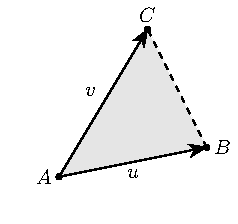
\includegraphics[width=0.6\linewidth]{figures/triangle.pdf}
  \end{figure}

  \noindent
  \paragraph{Example:}
  In particular, for the interior of a triangle, characterized by the points $A,B,C\in\setReal^3$, the first fundamental form is constant and we can set $u$ and $v$ as follows to use the above formulas.
  \[
    u\define B-A
    \separate
    v\define C-A
  \]
  To represent the function $f$ in a discretized form for a computer, we will use a triangle mesh and will only provide a value for each vertex.
  For interior points $x$ of triangles with barycentric coordinates $α,β,γ\in[0,1]$ with $α+β+γ=1$, linear interpolation over the vertex values $f(A)$, $f(B)$, and $f(C)$ is taken out.
  \[
    f(x) = α f(A) + β f(B) + γ f(C)
  \]
  As a result, the graph of the discretized function of $f$ is a plane for the interior of each triangle.
  So also its gradient is constant within the interior.
  Computing directional derivatives for $u$ and $v$ then reduces to the following expressions.
  \[
    \partial_u f = f(B)-f(A)
    \separate
    \partial_v f = f(C)-f(A)
  \]
  Applying these formulas for each triangle and accumulating those values at their vertices will give us an approach to estimate the gradients and directional derivatives on triangle meshes.

  % \begin{figure}
  %   \centering
  %   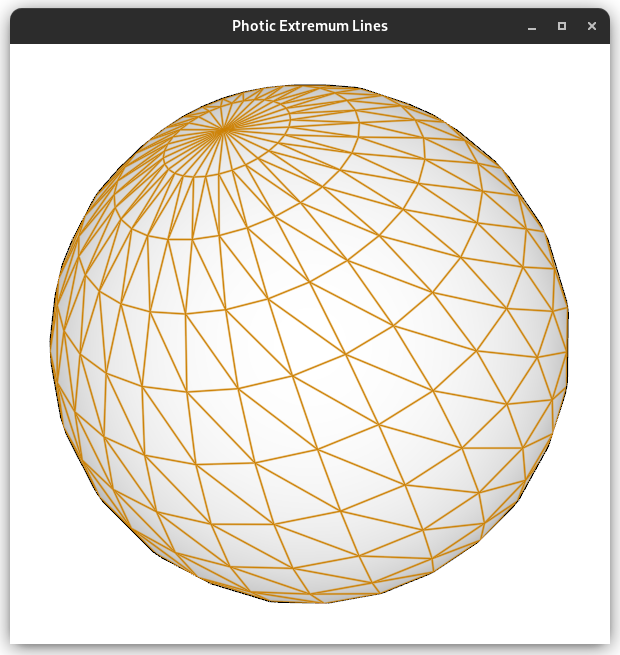
\includegraphics[width=0.6\linewidth,trim={15px 15 15 50},clip]{images/sphere-wireframe.png}
  %   \caption{Triangulated Meshes}
  % \end{figure}

\section{Photic Extremum Lines}

  \begin{figure*}[h]
    \centering
    \begin{subfigure}[b]{0.24\textwidth}
      \centering
      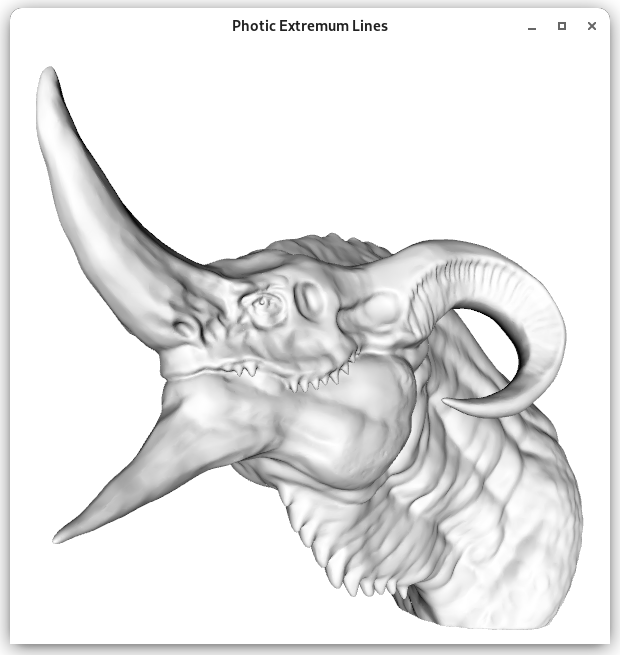
\includegraphics[width=0.95\textwidth,trim={15px 15 15 50},clip]{images/dragon-head-vertex-lighting.png}
      \caption{Illumination φ}
    \end{subfigure}%
    \hfill%
    \begin{subfigure}[b]{0.24\textwidth}
      \centering
      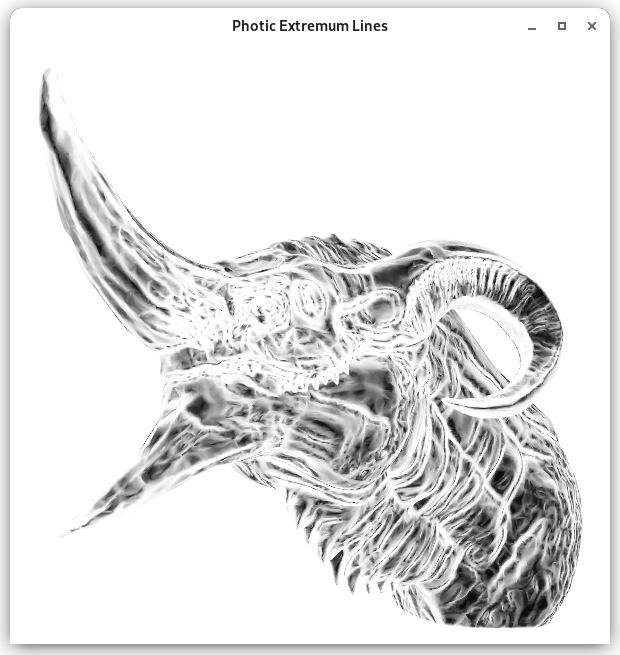
\includegraphics[width=0.95\textwidth,trim={15px 15 15 50},clip]{images/dragon-head-light-variation.png}
      \caption{Variation $\norm{\nabla{φ}}$}
    \end{subfigure}%
    \hfill%
    \begin{subfigure}[b]{0.24\textwidth}
      \centering
      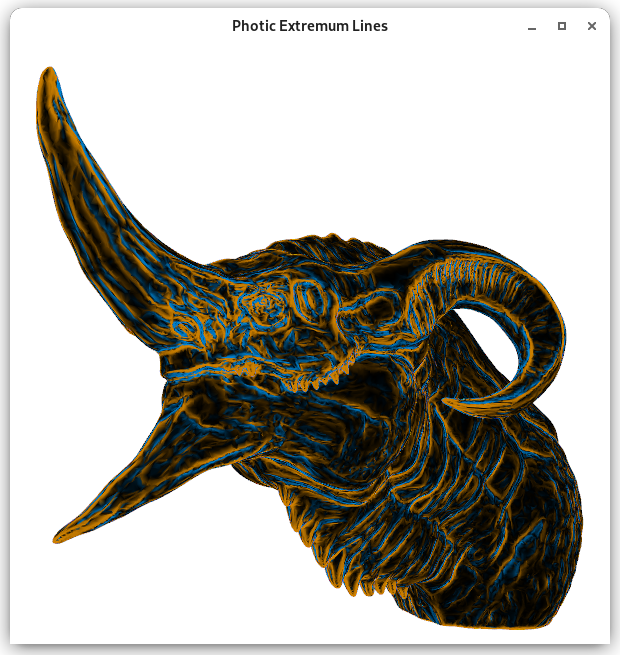
\includegraphics[width=0.95\textwidth,trim={15px 15 15 50},clip]{images/dragon-head-light-variation-slope.png}
      \caption{$\mathscr{D}_φ\norm{\nabla φ}$}
    \end{subfigure}%
    \hfill
    \begin{subfigure}[b]{0.24\textwidth}
      \centering
      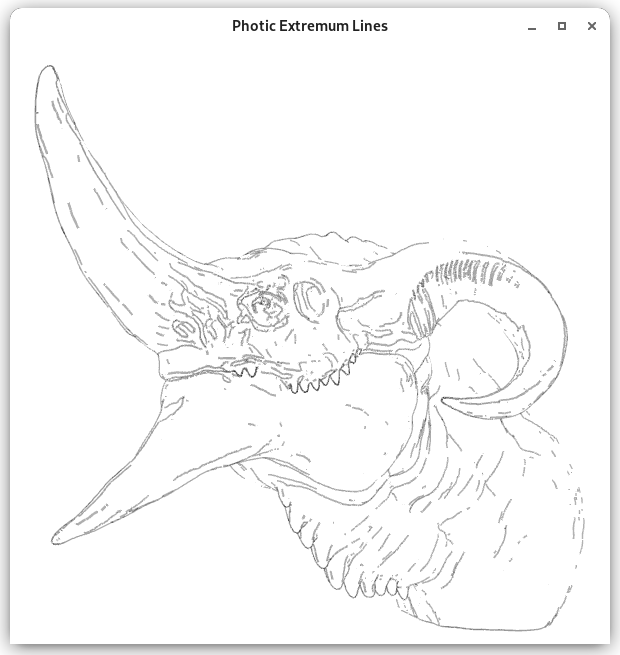
\includegraphics[width=0.95\textwidth,trim={15px 15 15 50},clip]{images/dragon-head-pel-shader.png}
      \caption{$\mathrm{PEL}_τ(S,φ)$}
    \end{subfigure}%
    \caption{%
      \textbf{Visualization of PEL Definition}\\
      These images show the same object with surface $S$.
      For each image, the object is shaded with a specific function or set of the PEL definition.
      Hereby, (c) uses orange for positive, blue for negative, and black for zero values.
      The images shall give an intuition on why the definition of PELs makes sense.
    }
    \label{fig:pel-definition-visualization}
  \end{figure*}

  Providing the mathematical details, now, we are in a position to give a formal definition of PELs.
  For this section, let $S$ again be a smooth surface patch and $\function{φ}{S}{\setReal}$ a three-times continuously differentiable scalar function that describes the illumination of the surface $S$ in grayscale values.

  \begin{definition*}[(Photic Extremum Lines)]
    The set $\mathrm{PEL}(S,φ)$ of photic extremum lines consists of all points $x\in S$ such that
    \[
      \mathscr{D}_φ\norm{\nabla φ}(x) = 0
      \separate
      \mathscr{D}^2_φ\norm{\nabla φ}(x) < 0
      \ .
    \]
    Such points are also called photic extrema.

    \smallskip
    Let $τ\in\setReal^+_0$ be an arbitrary threshold and $\mathscr{F}_τ(S,φ)$ a filter in the following sense.
    \[
      \mathscr{F}_τ(S,φ) \define \set{x\in S}{\norm{\nabla φ}(x) > τ}
    \]
    Then the set of τ-filtered photic extremum lines is defined as follows.
    \[
      \mathrm{PEL}_τ(S,φ) \define \mathrm{PEL}(S,φ)\cap\mathscr{F}_τ(S,φ)
    \]
  \end{definition*}

  \noindent
  In other words, photic extrema are points $x\in S$ where the variation of illumination $\norm{\nabla φ}$ in the direction $\nabla φ$ of its gradient reaches a local maximum.
  The definition involves the previously defined PEL operator to provide sufficient conditions for these specific local maxima.
  Figure \ref{fig:pel-definition-visualization} visualizes the different functions used in the above definition.

  Our definition strongly complies with the original definition given in \textcite{xie2007}.
  But additionally, we already added the threshold to point-wise filter out parts of lines that are too weak in the sense of light variation.
  This was mainly done to be mathematically rigorous in further discussions but also allows for more generalized filter techniques.
  The filtering is defined according to \textcite{zhang2010} to be able to achieve real-time performance.
  The original threshold filter method used in \textcite{xie2007} is based on a line tracing approach of \textcite{ohtake2004} and, as a consequence, is much more involved than the point-wise approach and would most likely lead to a bottleneck in the following algorithm.

  Due to the deliberately built-in dependence on illumination in the definition of PELs, we at last need to clarify which lighting model to choose.
  As touched in the introduction, in general, arbitrary illumination functions are allowed.
  The main problem is that not all known lighting models will result in near-natural line drawings.
  The comparison of different models would fill an article for itself and therefore is not in the scope of this report.
  For our purposes and according to \textcite{xie2007}, we will choose a simplified Phong model without ambient or specular lighting.
  In this way, only diffuse lighting, that depends on the cosine of the angle between the lighting direction and the normal of the surface, is allowed.
  Ambient lighting can be ignored as its directional derivatives would be zero.
  Since specular lighting effects only arise in small areas and greatly increase illumination, they would most likely introduce unnatural and artificial lines.

  Regarding the count and positioning of light sources, we again want to reduce the set of possibilities to make their specification feasible for this report.
  Therefore, only one light source will be used.
  Using this source with movements independent from the camera, PELs would not exhibit the wanted view dependency that other feature line types provide.
  Hence, we will position a directional light at the camera position such that light direction and view direction coincide.
  Due to the higher flexibility of PELs, only these restrictions make the results comparable to other feature lines not offering any kind of light dependence.

\section{Algorithm}
  The formal definition of PELs when put together with the basic techniques of \textcite{isenberg2003} and \textcite{rusinkiewicz2004} described in section \ref{sec:related-work} already supplies us with an intuitive approach to generate PELs.
  In the following, we will give the details.
  This time, let $\mathscr{M}=(V,E,F)$ be a regular triangle mesh consisting of vertices $V$, edges $E$, and faces $F$ that approximates a smooth two-dimensional surface.
  Furthermore, let $\function{n}{V}{\mathscr{S}^2}$ be the function that provides consistent and normalized normals for each vertex of $\mathscr{M}$.
  Let $S\define V\cup E\cup F$ be the surface of $\mathscr{M}$ and $\function{φ}{S}{\setReal}$ a scalar triangle mesh function representing the grayscale illumination of $\mathscr{M}$ with given values at each vertex which uses linear interpolation based on barycentric coordinates for edges and faces.

  \subsection{Overview}
  \label{sec:algorithm-overview}
    The whole PEL algorithm has to be executed each time the view position or lighting changes.
    This is in contrast to other feature lines that may precompute most of their needed information which are only based on surface geometry.

    Concerning time and effort, the main part of the algorithm needs to compute all the illumination derivatives $\nabla φ$, $\mathscr{D}_φ\norm{\nabla φ}$, and $\mathscr{D}^2_φ\norm{\nabla φ}$ for each vertex $v\in V$.
    Afterwards, an iteration over all edges $[v,w]\in E$ detects photic extrema on edges.
    Finally, an iteration over all faces $f\in F$ connects two feature line vertices of adjacent edges if present generating feature line segments.
    At last, the occlusion, threshold $τ\in\setReal_0^+$, and the value of $\norm{\nabla φ}$ for each point decide if the respective photic extremum represented by a fragment will be rendered.

    \begin{tcolorbox}[%
      colframe=black,
      colbacktitle=white,
      coltitle=black,
      colback=mathdefback,
      attach boxed title to top center={yshift=-2mm},
      enhanced,
      titlerule=0.1pt,
      boxrule=0.5pt,
      arc=5pt,
      breakable,
      width=\linewidth,
      title=Algorithm Overview
    ]
      \begin{enumerate}
        \item Compute $φ$ at each vertex
        \item Compute $\norm{\nabla φ}$ and $\frac{\nabla φ}{\norm{\nabla φ}}$ at each vertex
        \item Compute $\mathscr{D}_φ\norm{\nabla φ}$ at each vertex
        \item Compute $\mathscr{D}^2_φ\norm{\nabla φ}$ at each vertex
        \item Detect photic extrema on edges
        \item Emit feature line segment for each triangle with photic extrema on adjacent edges
        \item Discard fragments of feature lines \\ based on threshold
        \item Render non-occluded feature line \\ fragments by using hidden line removal
      \end{enumerate}
    \end{tcolorbox}

    \noindent
    In our implementation, points 1 to 4 are taken out on the CPU.
    Point 5 and 6 have been merged and put inside a geometry shader of the graphics pipeline.
    This makes it possible to implement the threshold-based discarding of PEL fragments inside a fragment shader by a simple branch comparing the illumination variation of the fragment to the given threshold.

  \subsection{Preprocessing}
    Besides loading the triangle mesh to be rendered with PELs, we have to generate the interpolated normals for every vertex if they are not already present.
    For this, we refer to the standard procedures given by \textcite{max1999} and \textcite{jin2005}.
    This may already be sufficient for triangle meshes that were created manually by graphic designers.
    Usually, such models provide us with very smooth surface normals.
    An example can be seen in figure \ref{fig:preprocessing-normals-smooth}.
    The car has been manually modeled and provides very smooth normals.
    And as a result, it shows a  near-perfect feature line extraction.

    \begin{figure}[h]
      \centering
      \begin{subfigure}[b]{\linewidth}
        \centering
        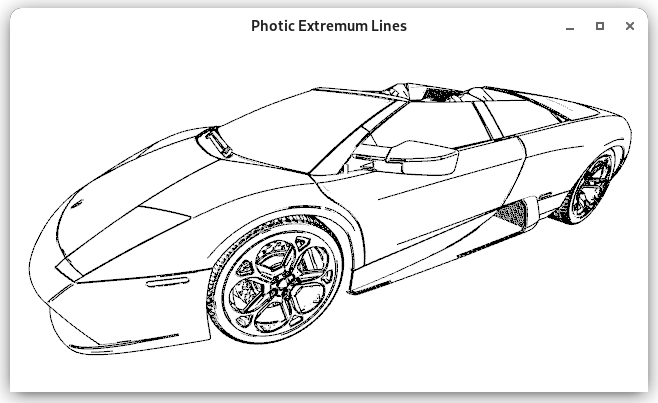
\includegraphics[width=\textwidth,trim={15px 15 15 50},clip]{images/lamborghini-front.png}
        \caption{Front}
      \end{subfigure}
      \begin{subfigure}[b]{\linewidth}
        \centering
        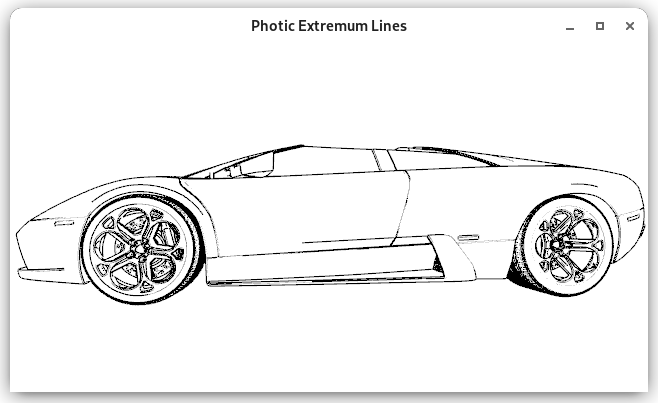
\includegraphics[width=\textwidth,trim={15px 15 15 50},clip]{images/lamborghini-side.png}
        \caption{Side}
      \end{subfigure}
      \caption{%
        \textbf{Nearly Perfect PEL Extraction for Smooth Normals}\\
        The images show different perspectives of the extracted PELs for the Lamborghini model that provides very smooth surface normals.
        It can be seen that the smoothness allows for a nearly perfect line extraction without artifacts.
      }
      \label{fig:preprocessing-normals-smooth}
    \end{figure}

    For triangle meshes originated from 3D scanners on the other hand, generated normals may be inaccurate due to errors in measurement or round-off errors.
    Such inconsistencies are typically called noise and would probably result in artifacts when rendering feature lines because derivative computations have a major dependency on surface normals.
    The effects can be seen in figure \ref{fig:preprocessing-normals-noise}.
    As a consequence, further preprocessing would involve reducing the noise of such normals by using bilateral normal filtering for example as it was done in \textcite{xie2007}.
    Here, we will not provide any details concerning this topic because such filters need parameters that may be tweaked by the user.

    \begin{figure}[h]
      \centering
      \begin{subfigure}[b]{0.49\linewidth}
        \centering
        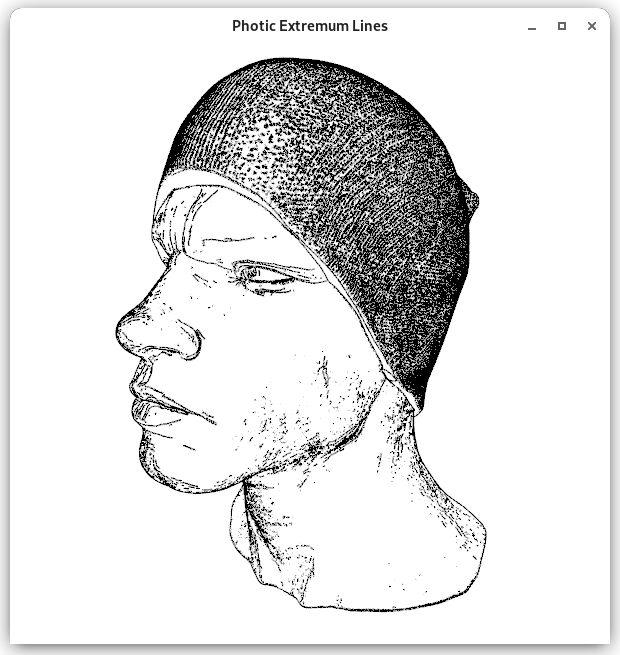
\includegraphics[width=\textwidth,trim={15px 15 15 50},clip]{images/head-contour-pel-shader.png}
        \caption{Contours and PELs}
      \end{subfigure}
      \begin{subfigure}[b]{0.49\linewidth}
        \centering
        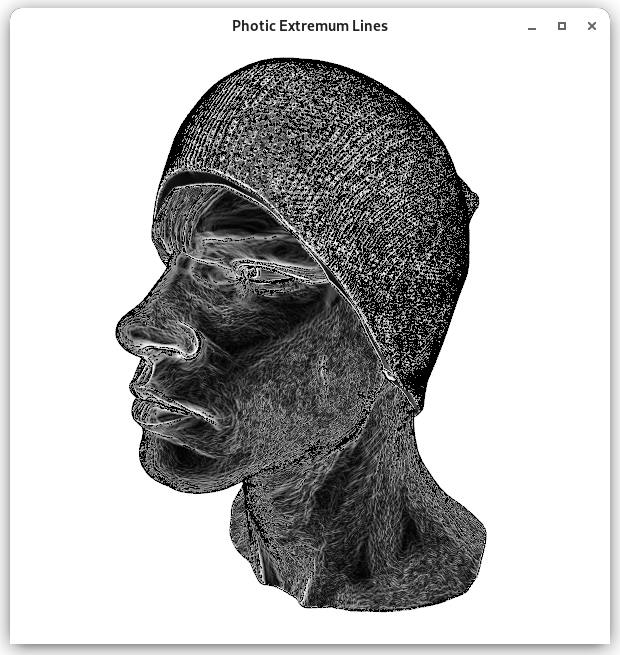
\includegraphics[width=\textwidth,trim={15px 15 15 50},clip]{images/head-light-variation.png}
        \caption{Variation}
      \end{subfigure}
      \caption{%
        \textbf{Erroneous PEL Extraction for Noisy Normals}\\
        The images show extracted PELs and light variation of the head model.
        This model provides very noisy surface normals which manifest in PEL artifacts around the chin and neck.
        The light variation visualizes the noise of the surface normals.
      }
      \label{fig:preprocessing-normals-noise}
    \end{figure}

    For the computation of gradients and directional derivatives on the triangle mesh, each vertex should be equipped with an orthonormal system of two vectors spanning its tangent space.
    Generating such tangent vectors can be quite arbitrary.
    Our approach first uses a uniform distribution on the unit sphere to randomly generate normalized directions for each vertex.
    In conjunction with the vertex normal, we can then compute these tangent space vectors by two cross products.

    \textcite{rusinkiewicz2004}, \textcite{xie2007}, and \textcite{zhang2010} all refer to \textcite{meyer2001} when it comes to the accumulation step of face gradients at their vertices.
    Hereby, each gradient or directional derivative is weighted based on the Voronoi area of the point inside the current triangle with respect the whole Voronoi area of the vertex.
    As a consequence, these Voronoi weights should also be precomputed and stored with respect to their vertices and faces.
    % Additionally, neighboring vertices should be stored for parallelization.

  \subsection{Gradient Computation}
    As said in section \ref{sec:algorithm-overview}, the main part of the algorithm needs to compute all the illumination derivatives.
    All of these can be computed with the same approach.

    For each face, compute the constant gradient by using formula in background.
    Transform and rotate this gradient into the local vertex system and accumulate multiplied with Voronoi weight.
    Afterwards iterate over all vertices for normalization.

    \begin{tcolorbox}[%
      colframe=black,
      colbacktitle=white,
      coltitle=black,
      colback=mathdefback,
      attach boxed title to top center={yshift=-2mm},
      enhanced,
      titlerule=0.1pt,
      boxrule=0.5pt,
      arc=5pt,
      breakable,
      width=\linewidth,
      title=Gradient Algorithm
    ]
      \begin{enumerate}
        \item For each face, compute gradient in $uv$-coordinate representation
        \item For each adjacent vertex, transform representation into local $uv$-coordinates
        \item for directional derivatives, compute them at vertices
        \item Accumulate this representation by using Voronoi weights
      \end{enumerate}
    \end{tcolorbox}

  \subsection{Line Extraction}
    In section \ref{sec:algorithm-overview}, an overview of the PEL algorithm was given.
    Here, the details for an implementation of points 5 and 6 are provided.
    The subpolygon feature line extraction method is a general method for object-space feature line algorithms described in \textcite{isenberg2003} and \textcite{xie2007}.
    The following snippet summarizes the main points.
    Hereby, we define the following short notation.
    \[
      h(x)\define\mathscr{D}_φ\norm{\nabla φ}(x)
    \]

    \begin{tcolorbox}[%
      colframe=black,
      colbacktitle=white,
      coltitle=black,
      colback=mathdefback,
      attach boxed title to top center={yshift=-2mm},
      enhanced,
      titlerule=0.1pt,
      boxrule=0.5pt,
      arc=5pt,
      breakable,
      width=\linewidth,
      title=PEL Extraction
    ]
      \begin{enumerate}
        \item For each edge $[v,w]\in E$:
        \begin{enumerate}
          \item Check for zero-crossing:
          \[
            h(v)h(w) < 0
          \]
          \item If this is the case, \\ approximate zero-crossing:
          \[
            p \define \frac{\absolute{h(w)}v + \absolute{h(v)}w}{\absolute{h(v)} + \absolute{h(w)}}
          \]
          \item Check maximum condition:
          \[
            \mathscr{D}_φ^2\norm{\nabla φ}(p) < 0
          \]
          \item If this is the case, \\ emit PEL vertex $p$
        \end{enumerate}
        \item For each triangle:
        \begin{enumerate}
          \item Check if two adjacent edges \\ provide PEL vertices $p$ and $q$
          \item If this is the case, \\ emit PEL segment $[p,q]$
        \end{enumerate}
      \end{enumerate}
    \end{tcolorbox}

    \noindent
    A close-up view of a result of this algorithm for a given triangle mesh is given in figure \ref{fig:subpolygon-feature-lines}.
    Here, every triangle whose edges exhibit a PEL vertex show a straight line segment connecting those vertices.
    Because neighboring triangles will compute the same PEL vertices on identical edges, in the overall result line segments are connected to whole feature lines.

    \begin{figure}[t]
      \centering
      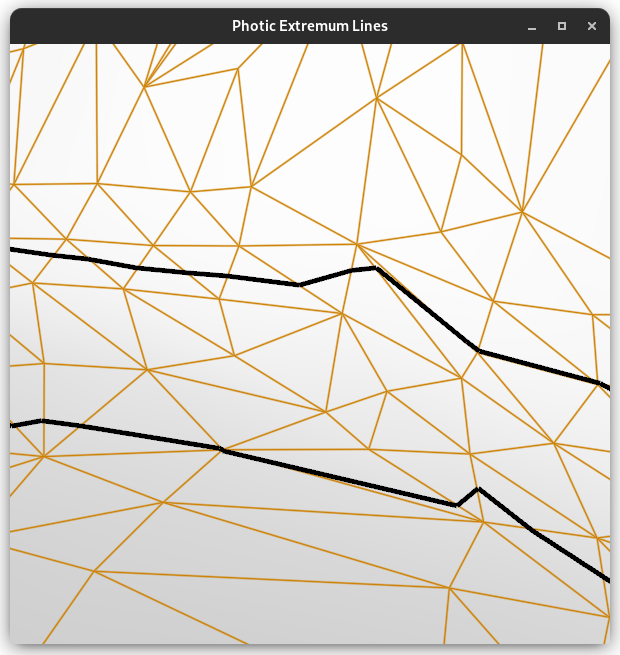
\includegraphics[width=0.8\linewidth,trim={15px 15 15 50},clip]{images/subpolygon-lines.png}
      \caption{%
        \textbf{Sub-Polygon Feature Lines}\\
        The image shows a close-up view of the mesh grid and PELs of a shaded triangle mesh.
        Each triangle whose adjacent edges exhibit PEL vertices show a straight line segment.
        As a result, neighboring triangles will connect line segments to a whole line.
      }
      \label{fig:subpolygon-feature-lines}
    \end{figure}

    As already described, the implementation of both points can be done in one single step by using the geometry shader of the graphics pipeline.
    For that matter, the input consists of triangles.
    For all edges of the given triangle, we will then do the steps provided in point 1 of the above algorithm.
    The geometry shader allows us to easily emit and render line segments.
    So each PEL vertex is at most computed twice but in a highly parallel approach on the GPU.
    This geometry shader implementation strongly aligns to the ideas given in \textcite{zhang2010}.

  \subsection{Hidden Line Removal}
    For themselves, feature line algorithms that work in object space in the first instance cannot decide which lines are occluded by the object's geometry since they have no concept of depth.
    Not removing occluded lines results in images like the one given in figure \ref{fig:hidden-line-removal}.
    There, we also see the correct variant where only non-occluded lines are shown.
    According to \textcite{isenberg2003}, this problem is typically referenced as \textit{hidden line removal} and can be dealt with by using several different techniques.

    \begin{figure}[h]
      \centering
      \begin{subfigure}[b]{0.49\linewidth}
        \centering
        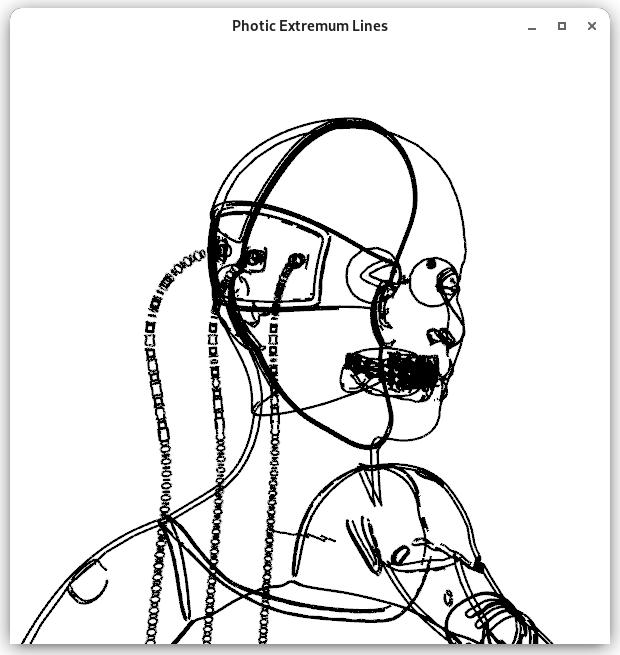
\includegraphics[width=\textwidth,trim={15px 15 15 50},clip]{images/cyborg-contour-pel-hidden-shader.png}
        \caption{Off}
      \end{subfigure}
      \begin{subfigure}[b]{0.49\linewidth}
        \centering
        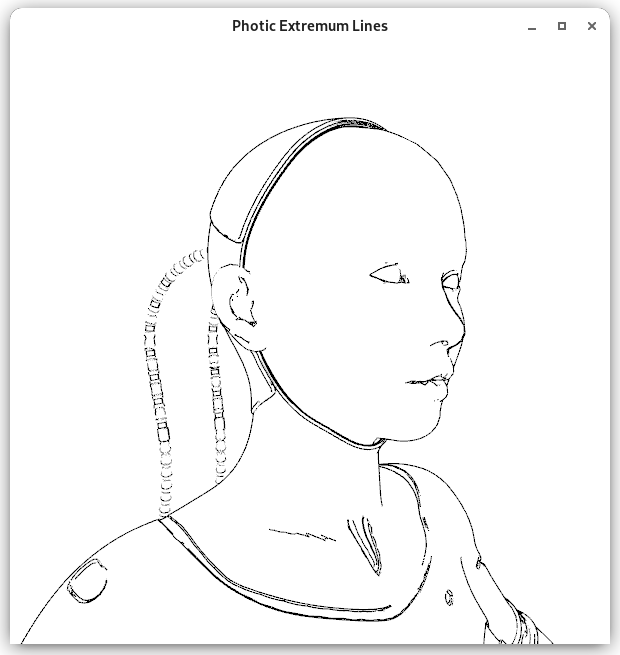
\includegraphics[width=\textwidth,trim={15px 15 15 50},clip]{images/cyborg-contour-pel-shader.png}
        \caption{On}
      \end{subfigure}
      \caption{%
        \textbf{Two-Pass Rendering for Hidden Line Removal}\\
        These images show the PELs of the same model.
        For the left image, a two-pass rendering approach to remove by the object's geometry occluded lines has not been used.
        For the image on the right, first, the whole uncolored surface was rendered to write into the depth buffer and afterwards the feature lines were drawn.
      }
      \label{fig:hidden-line-removal}
    \end{figure}

    Probably the simplest method involves using the depth buffer together with depth testing of the standard graphics pipeline.
    Hereby, the object will first be rendered as a whole but possibly uncolored surface.
    This makes sure that every fragment that can be seen from the camera stores its depth value into the depth buffer.
    All successive rendering calls will then test the depth values of their fragments against the depth buffer.
    In a second rendering pass, the extraction of feature lines will generate fragments with respective depth values.
    The built-in depth test will then discard such fragments that are occluded because their depth values are too high.

    Problems?

% \section{Implementation}

\section{Results}
  \subsection{Quality}

    \begin{figure*}
      \centering
      \begin{subfigure}[t]{0.19\textwidth}
        \centering
        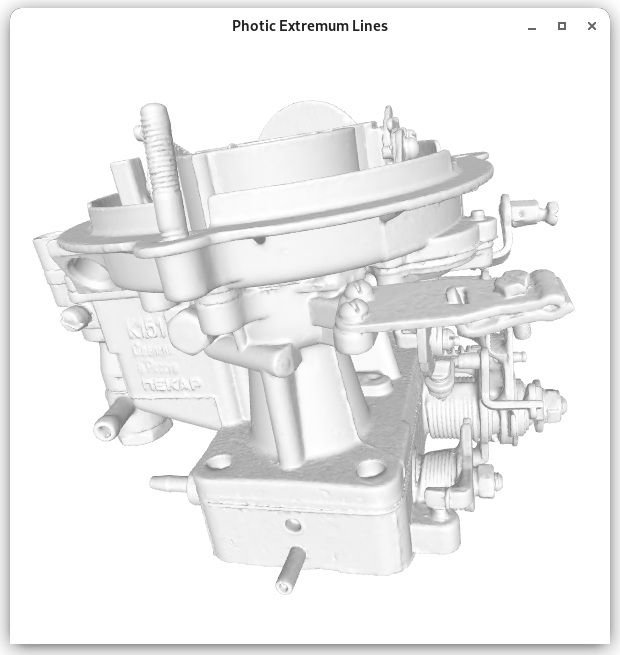
\includegraphics[width=0.95\textwidth,trim={15px 15 15 50},clip]{images/results/carburetor.png}
        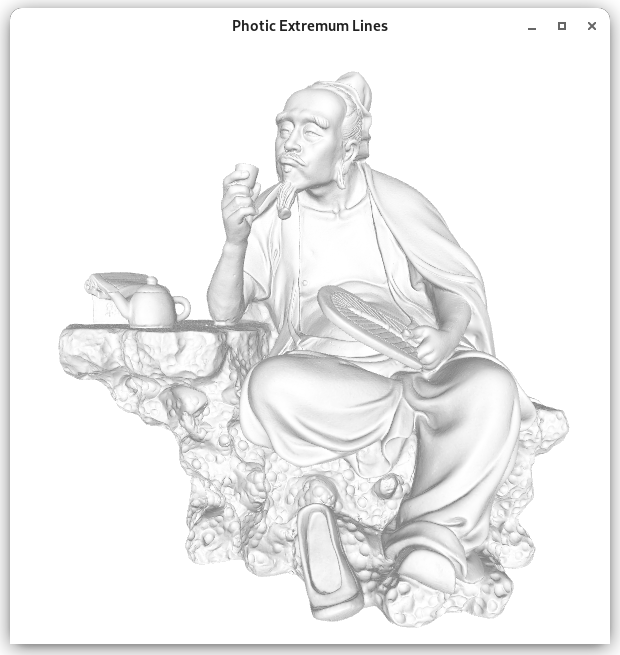
\includegraphics[width=0.95\textwidth,trim={15px 15 15 50},clip]{images/results/luyu.png}
        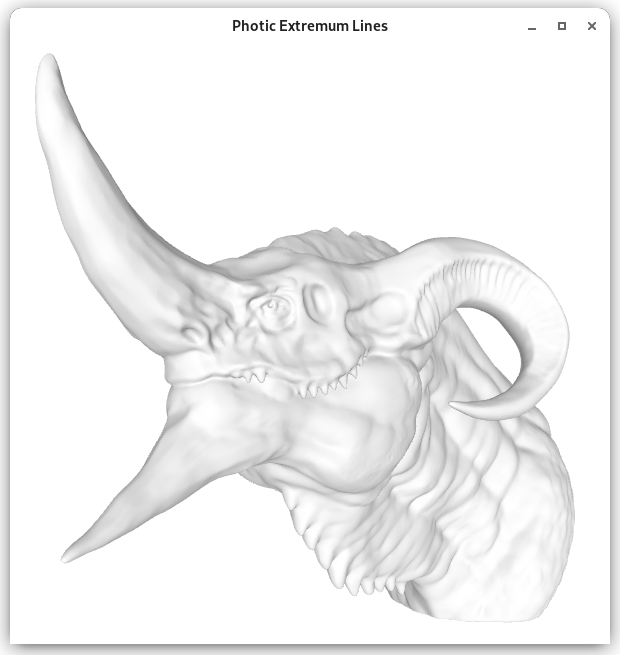
\includegraphics[width=0.95\textwidth,trim={15px 15 15 50},clip]{images/results/dragon-head.png}
        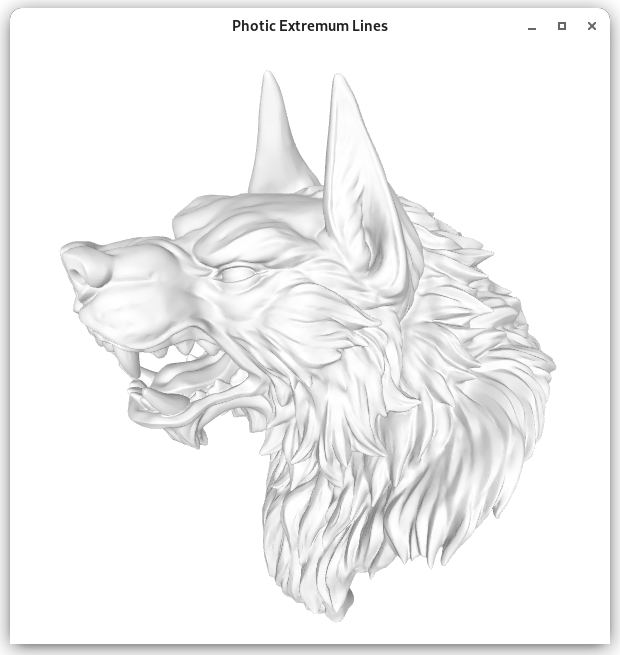
\includegraphics[width=0.95\textwidth,trim={15px 15 15 50},clip]{images/results/werewolf.png}
        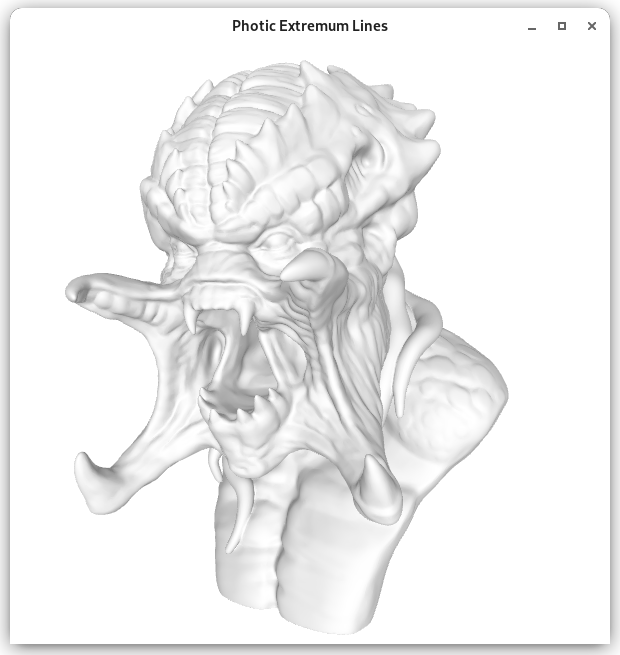
\includegraphics[width=0.95\textwidth,trim={15px 15 15 50},clip]{images/results/predator.png}
        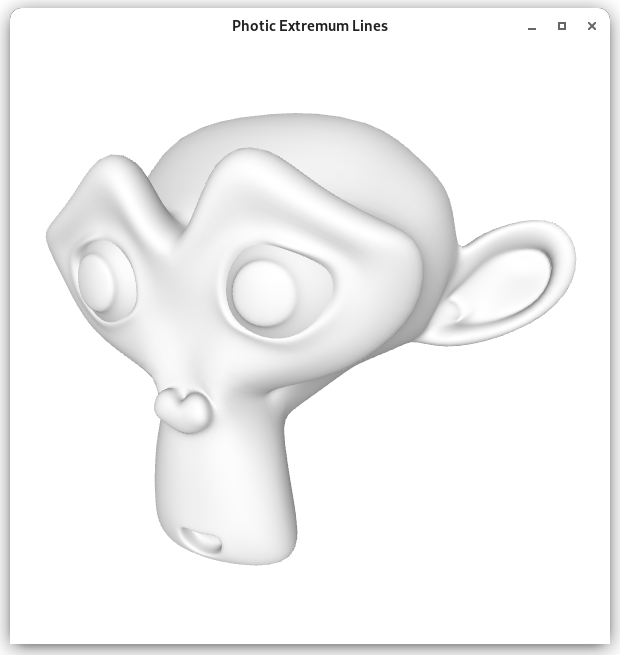
\includegraphics[width=0.95\textwidth,trim={15px 15 15 50},clip]{images/results/suzanne.png}
        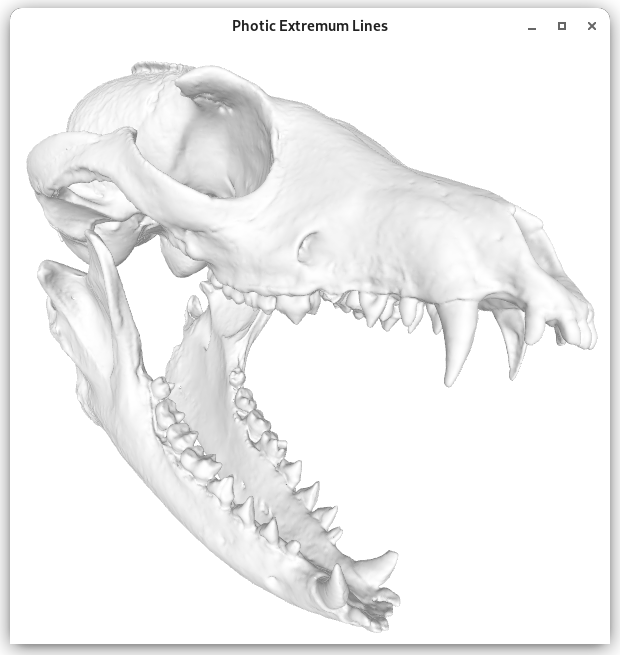
\includegraphics[width=0.95\textwidth,trim={15px 15 15 50},clip]{images/results/skull.png}
        \caption{Illumination}
      \end{subfigure}%
      \hfill%
      \begin{subfigure}[t]{0.19\textwidth}
        \centering
        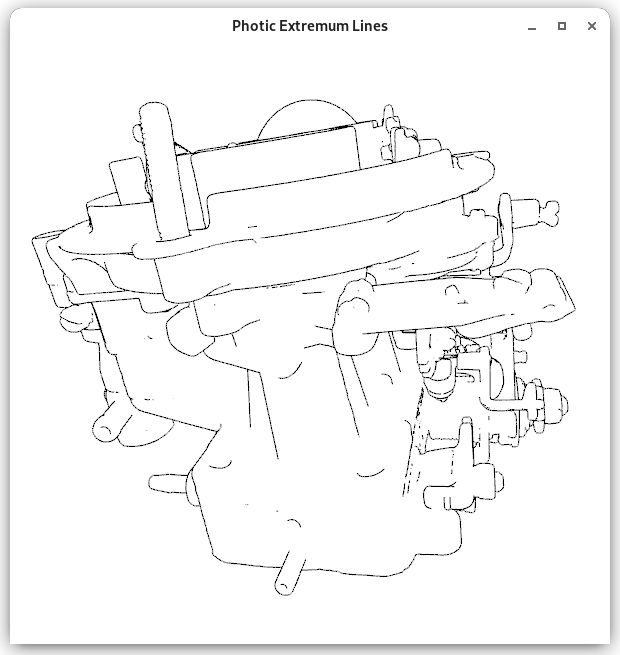
\includegraphics[width=0.95\textwidth,trim={15px 15 15 50},clip]{images/results/carburetor-contours.png}
        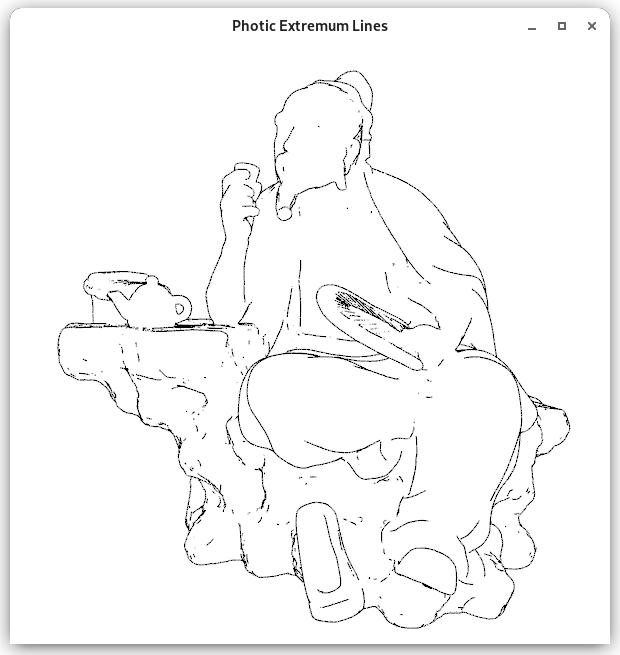
\includegraphics[width=0.95\textwidth,trim={15px 15 15 50},clip]{images/results/luyu-contours.png}
        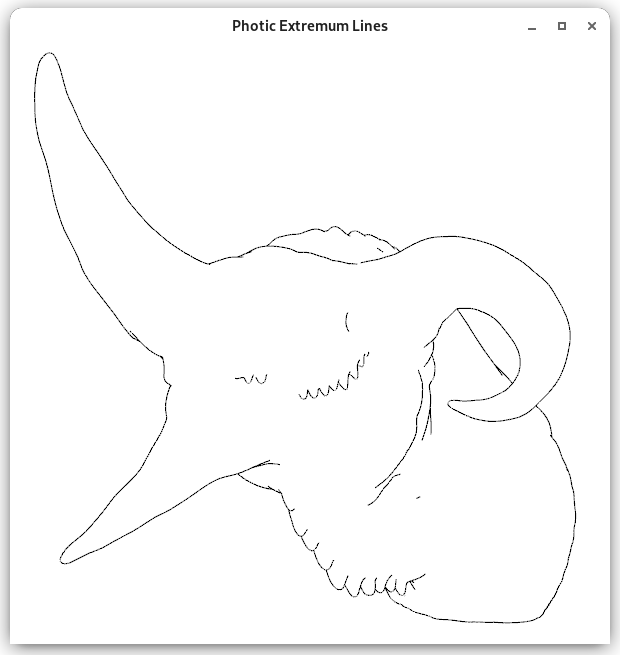
\includegraphics[width=0.95\textwidth,trim={15px 15 15 50},clip]{images/results/dragon-head-contours.png}
        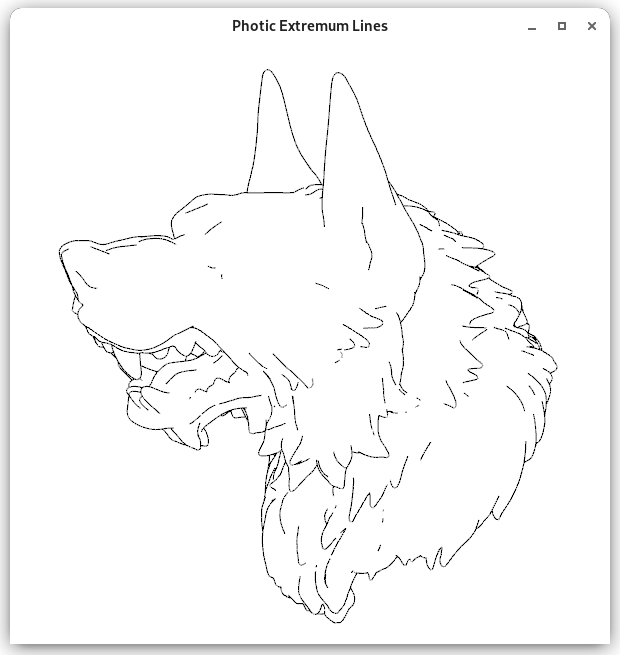
\includegraphics[width=0.95\textwidth,trim={15px 15 15 50},clip]{images/results/werewolf-contours.png}
        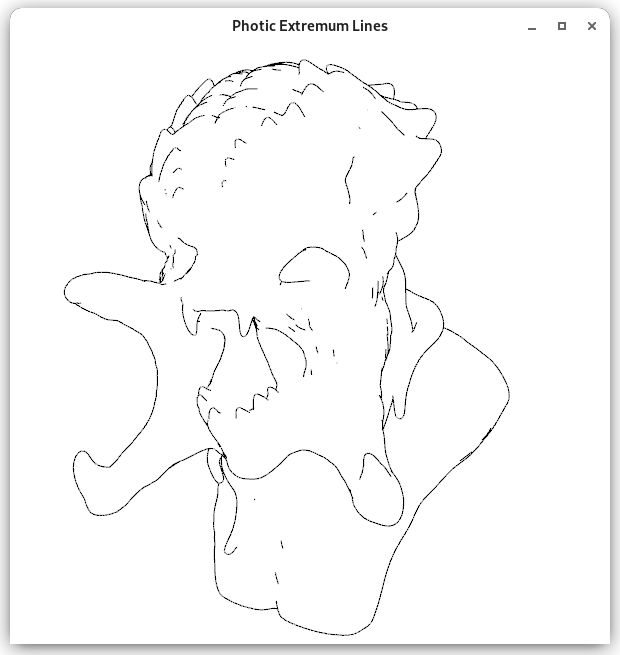
\includegraphics[width=0.95\textwidth,trim={15px 15 15 50},clip]{images/results/predator-contours.png}
        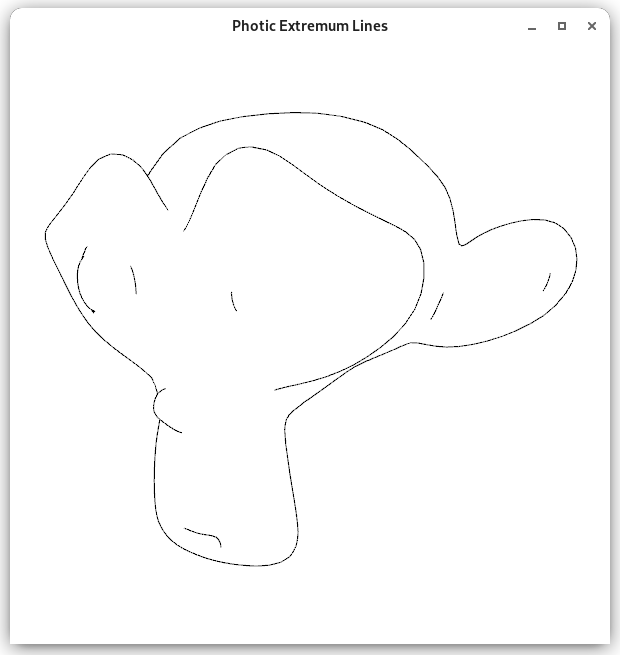
\includegraphics[width=0.95\textwidth,trim={15px 15 15 50},clip]{images/results/suzanne-contours.png}
        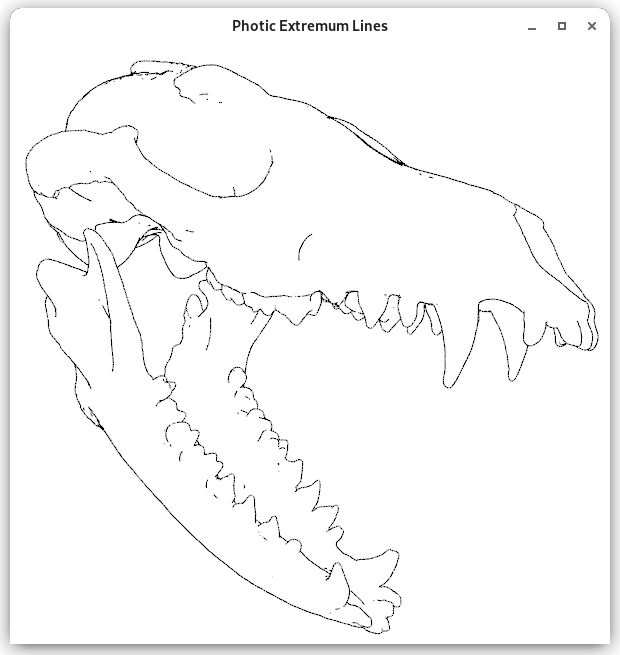
\includegraphics[width=0.95\textwidth,trim={15px 15 15 50},clip]{images/results/skull-contours.png}
        \caption{Contours}
      \end{subfigure}%
      \hfill%
      \begin{subfigure}[t]{0.19\textwidth}
        \centering
        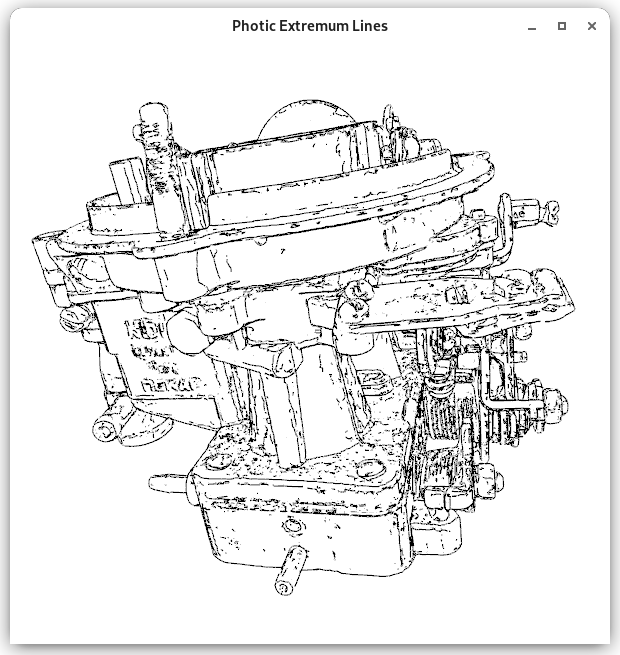
\includegraphics[width=0.95\textwidth,trim={15px 15 15 50},clip]{images/results/carburetor-pel.png}
        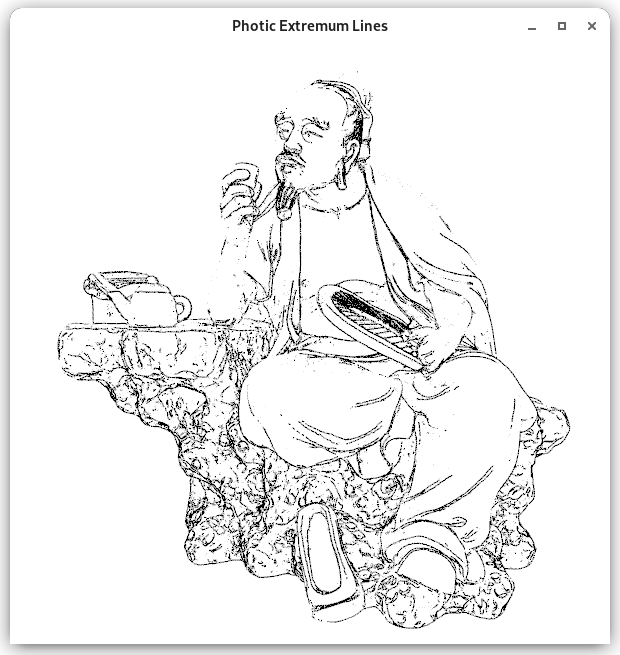
\includegraphics[width=0.95\textwidth,trim={15px 15 15 50},clip]{images/results/luyu-pel.png}
        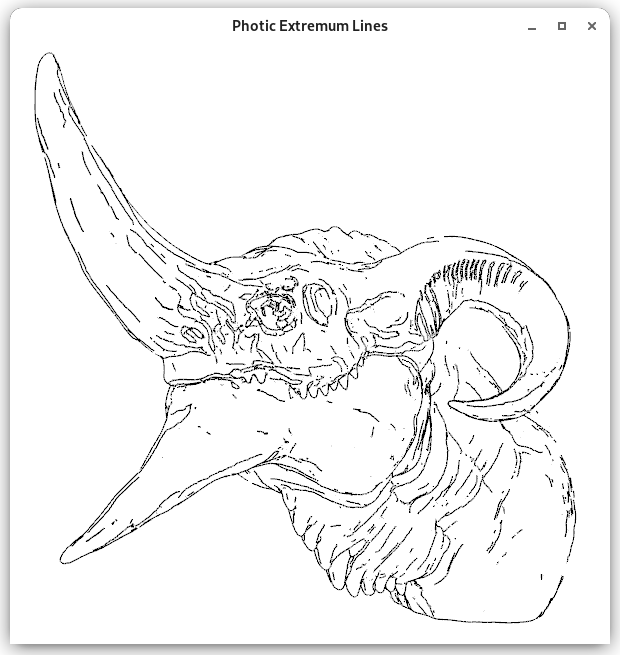
\includegraphics[width=0.95\textwidth,trim={15px 15 15 50},clip]{images/results/dragon-head-pel.png}
        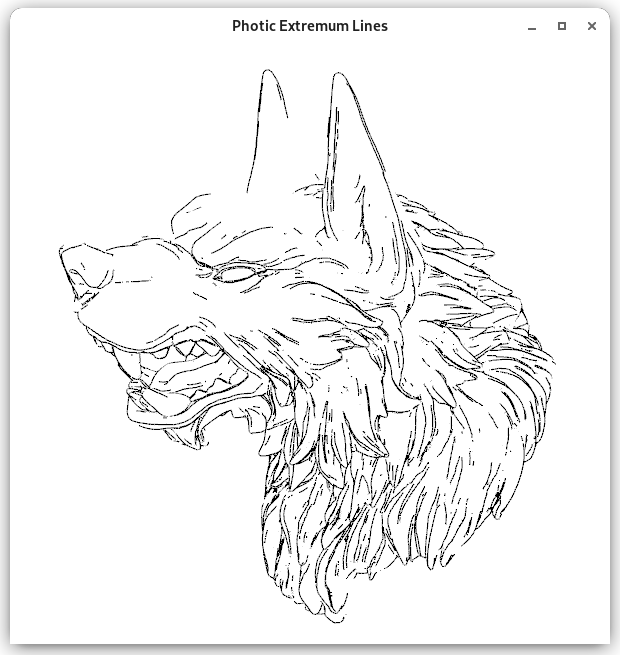
\includegraphics[width=0.95\textwidth,trim={15px 15 15 50},clip]{images/results/werewolf-pel.png}
        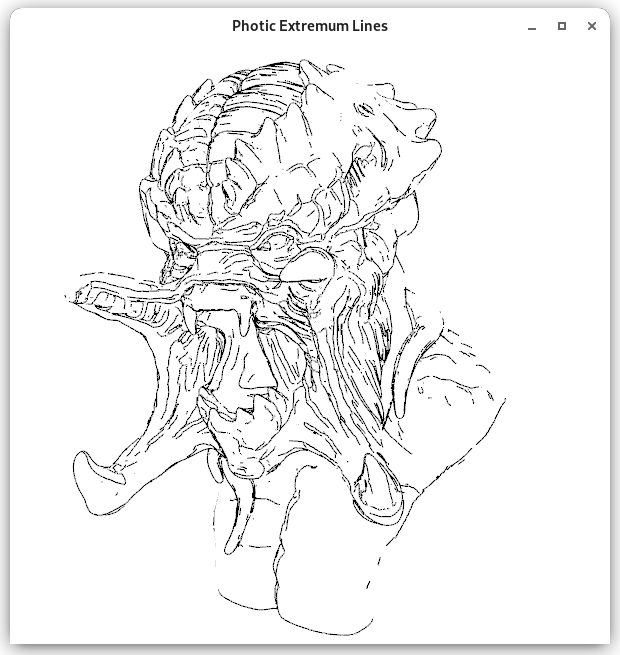
\includegraphics[width=0.95\textwidth,trim={15px 15 15 50},clip]{images/results/predator-pel.png}
        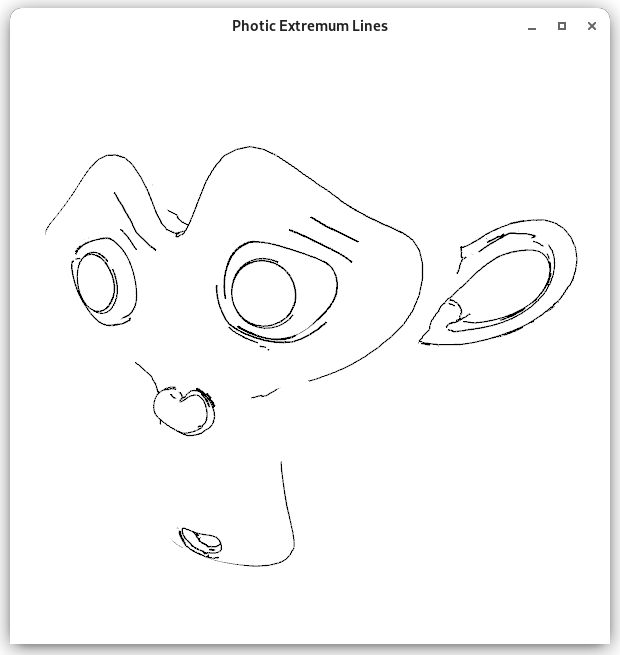
\includegraphics[width=0.95\textwidth,trim={15px 15 15 50},clip]{images/results/suzanne-pel.png}
        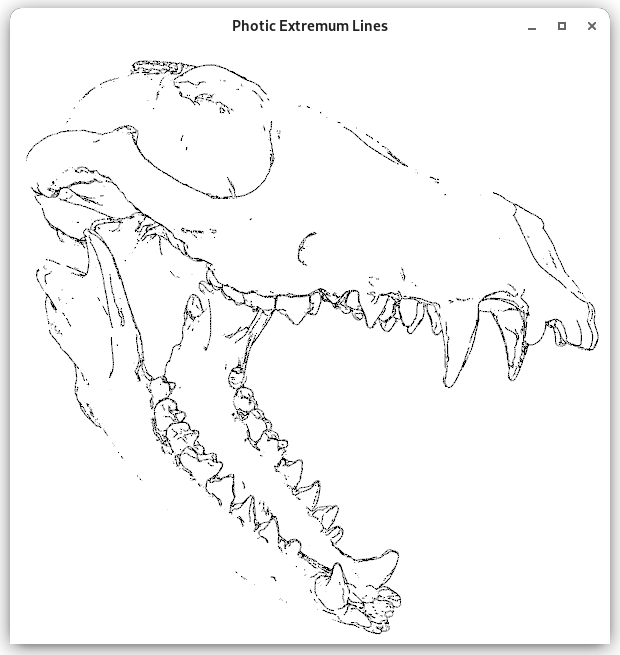
\includegraphics[width=0.95\textwidth,trim={15px 15 15 50},clip]{images/results/skull-pel.png}
        \caption{PELs}
      \end{subfigure}%
      \hfill
      \begin{subfigure}[t]{0.19\textwidth}
        \centering
        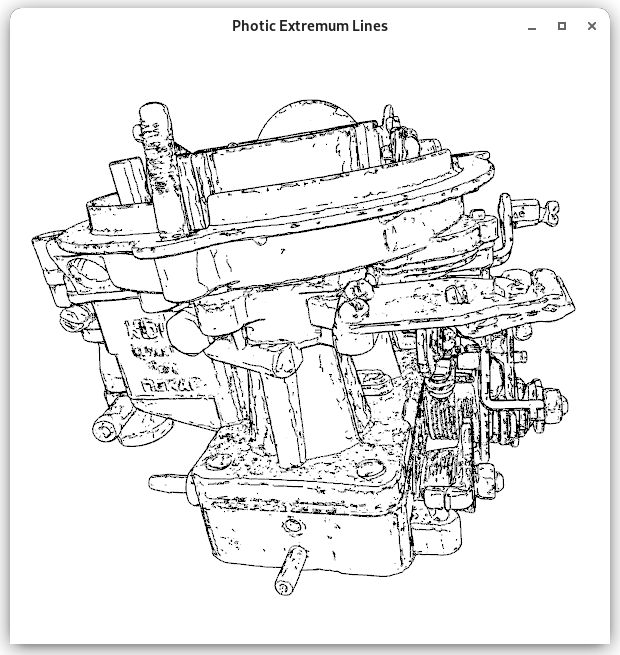
\includegraphics[width=0.95\textwidth,trim={15px 15 15 50},clip]{images/results/carburetor-contours-pel.png}
        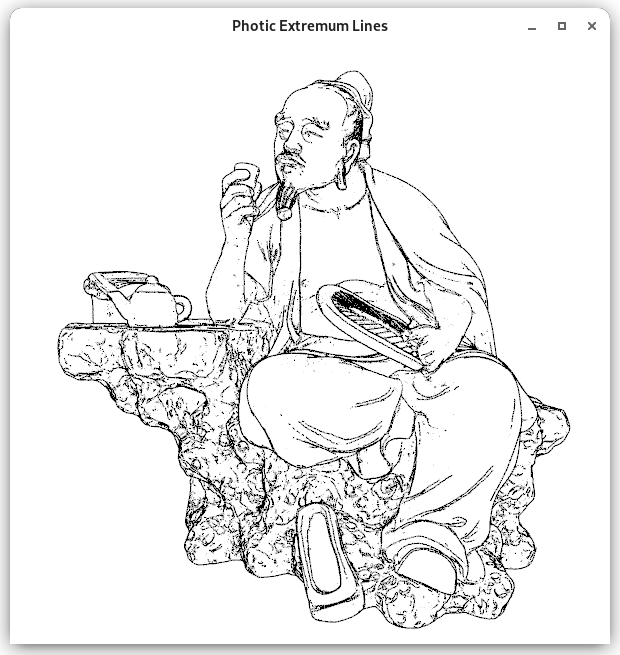
\includegraphics[width=0.95\textwidth,trim={15px 15 15 50},clip]{images/results/luyu-contours-pel.png}
        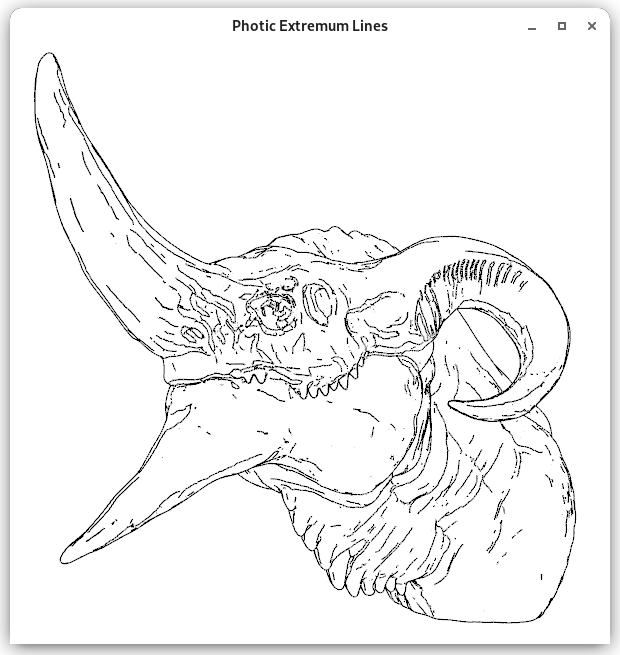
\includegraphics[width=0.95\textwidth,trim={15px 15 15 50},clip]{images/results/dragon-head-contours-pel.png}
        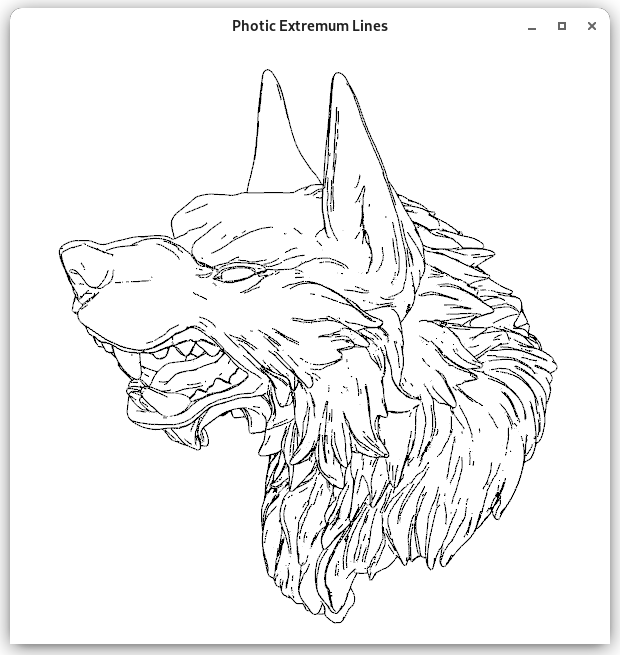
\includegraphics[width=0.95\textwidth,trim={15px 15 15 50},clip]{images/results/werewolf-contours-pel.png}
        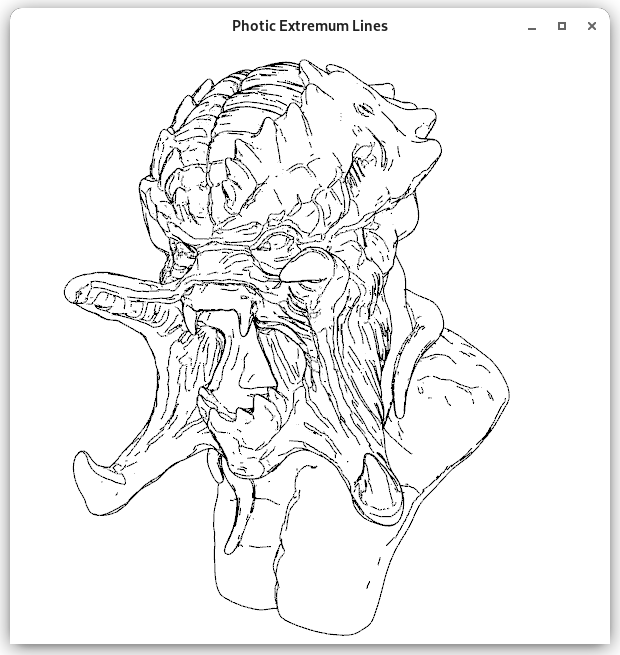
\includegraphics[width=0.95\textwidth,trim={15px 15 15 50},clip]{images/results/predator-contours-pel.png}
        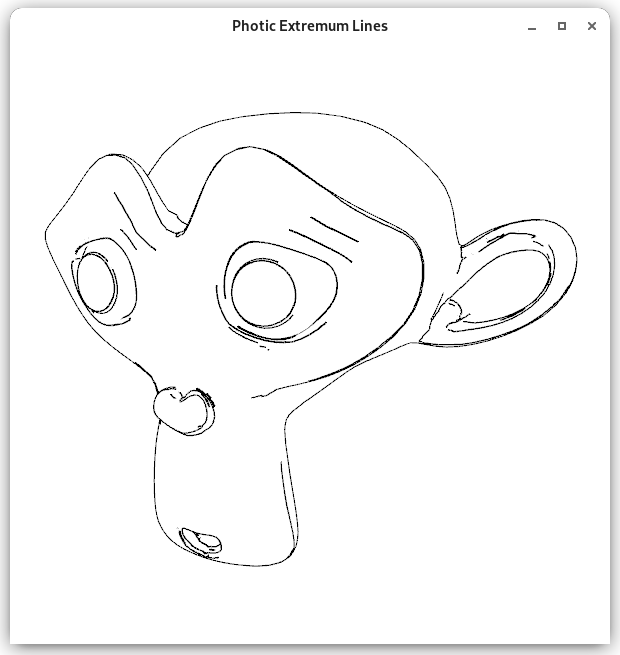
\includegraphics[width=0.95\textwidth,trim={15px 15 15 50},clip]{images/results/suzanne-contours-pel.png}
        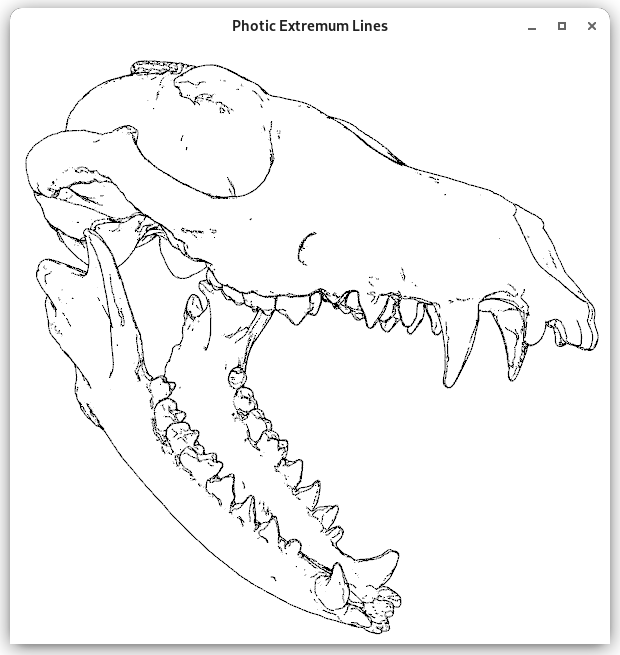
\includegraphics[width=0.95\textwidth,trim={15px 15 15 50},clip]{images/results/skull-contours-pel.png}
        \caption{Contours and PELs}
      \end{subfigure}%
      \hfill
      \begin{subfigure}[t]{0.19\textwidth}
        \centering
        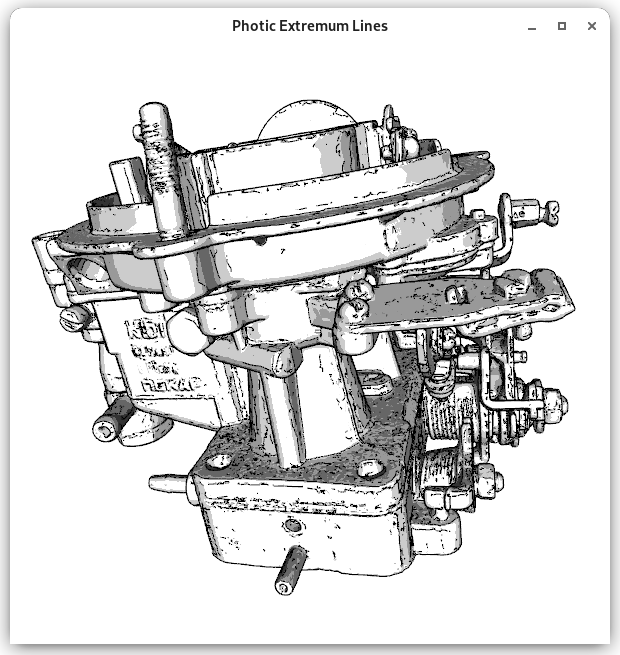
\includegraphics[width=0.95\textwidth,trim={15px 15 15 50},clip]{images/results/carburetor-contours-pel-toon.png}
        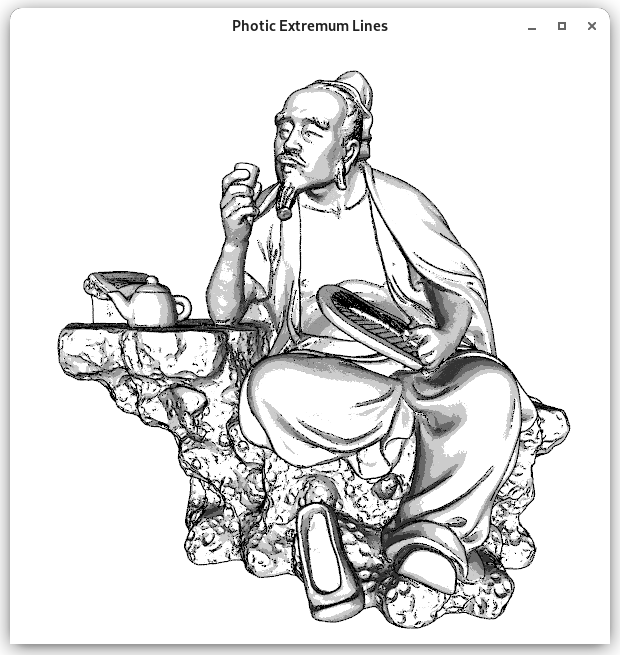
\includegraphics[width=0.95\textwidth,trim={15px 15 15 50},clip]{images/results/luyu-contours-pel-toon.png}
        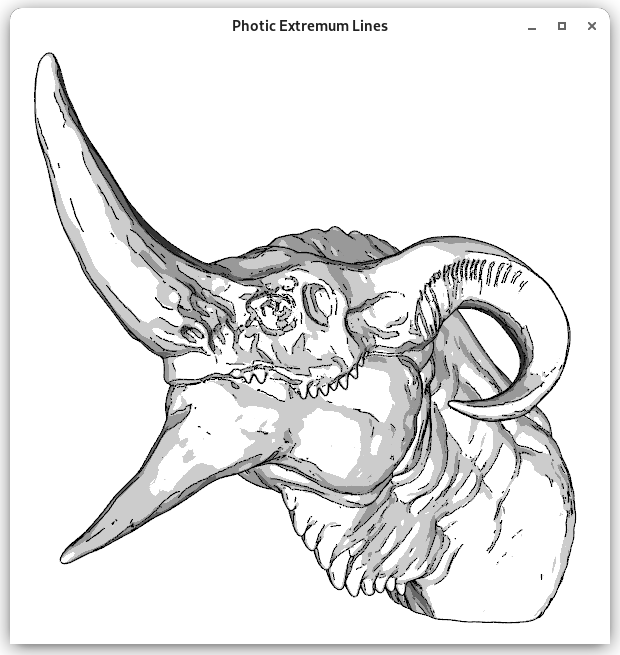
\includegraphics[width=0.95\textwidth,trim={15px 15 15 50},clip]{images/results/dragon-head-contours-pel-toon.png}
        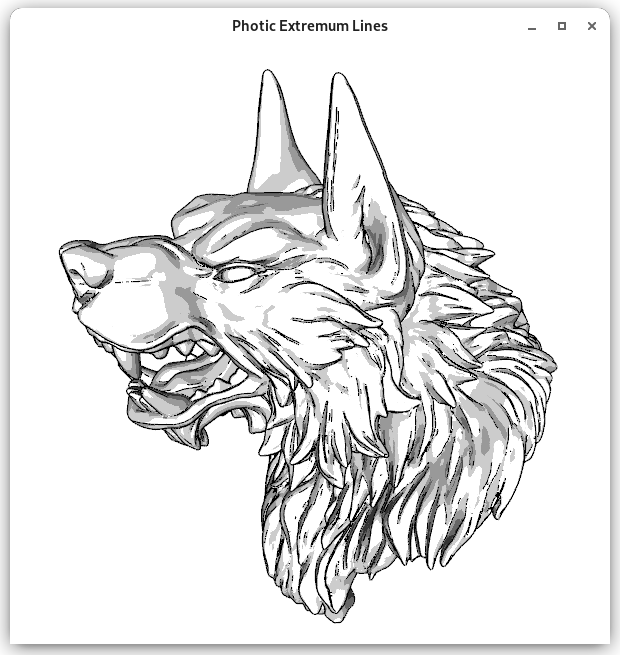
\includegraphics[width=0.95\textwidth,trim={15px 15 15 50},clip]{images/results/werewolf-contours-pel-toon.png}
        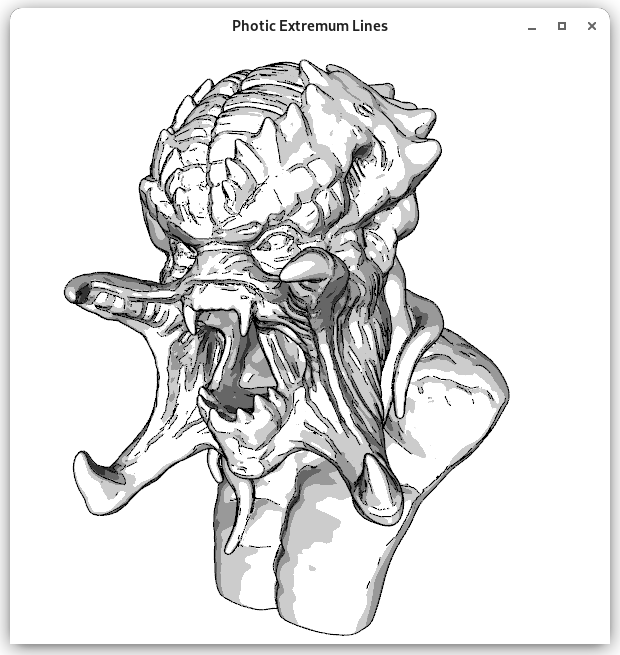
\includegraphics[width=0.95\textwidth,trim={15px 15 15 50},clip]{images/results/predator-contours-pel-toon.png}
        \includegraphics[width=0.95\textwidth,trim={15px 15 15 50},clip]{images/results/suzanne-contours-pel-toon.png}
        \includegraphics[width=0.95\textwidth,trim={15px 15 15 50},clip]{images/results/skull-contours-pel-toon.png}
        \caption{Toon Shader}
      \end{subfigure}%
      \caption{%
        \textbf{Quality Results}\\
        The images show the carburetor, lu yu, dragon head, werewolf, predator, suzanne, and fox skull models with varying shading models.
        The toon shading on the right is always done in conjunction with contours and PELs.
      }
      \label{fig:quality-results}
    \end{figure*}

  \subsection{Performance}

  lighting models and optimal lighting

  \begin{figure}[h]
    \centering
    \begin{subfigure}[b]{0.49\linewidth}
      \centering
      \includegraphics[width=\textwidth,trim={15px 15 15 50},clip]{images/fox-skull-threshold-low.png}
      \caption{Low}
    \end{subfigure}
    \begin{subfigure}[b]{0.49\linewidth}
      \centering
      \includegraphics[width=\textwidth,trim={15px 15 15 50},clip]{images/fox-skull-threshold-mid.png}
      \caption{Mid}
    \end{subfigure}
    \caption{Effect of thresholding}
  \end{figure}

  \begin{figure*}[h]
      \centering
      \begin{subfigure}[b]{0.24\textwidth}
        \centering
        \includegraphics[width=0.95\textwidth,trim={15px 15 15 50},clip]{images/dragon-head-viewer-shader.png}
        \caption{Illumination}
      \end{subfigure}%
      \hfill%
      \begin{subfigure}[b]{0.24\textwidth}
        \centering
        \includegraphics[width=0.95\textwidth,trim={15px 15 15 50},clip]{images/dragon-head-contours.png}
        \caption{Contours}
      \end{subfigure}%
      \hfill%
      \begin{subfigure}[b]{0.24\textwidth}
        \centering
        \includegraphics[width=0.95\textwidth,trim={15px 15 15 50},clip]{images/dragon-head-contour-pel-shader.png}
        \caption{Contours and PELs}
      \end{subfigure}%
      \hfill
      \begin{subfigure}[b]{0.24\textwidth}
        \centering
        \includegraphics[width=0.95\textwidth,trim={15px 15 15 50},clip]{images/dragon-head-contour-pel-toon-shader.png}
        \caption{Contours, PELs, and Toon}
      \end{subfigure}%
      \caption{\textbf{Short Summary Part}\\
      Lorem ipsum dolor sit amet, consectetur adipisicing elit, sed do eiusmod
      tempor incididunt ut labore et dolore magna aliqua. Ut enim ad minim veniam,
      quis nostrud exercitation ullamco laboris nisi ut aliquip ex ea commodo
      consequat. Duis aute irure dolor in reprehenderit in voluptate velit esse
      cillum dolore eu fugiat nulla pariatur. Excepteur sint occaecat cupidatat non
      proident, sunt in culpa qui officia deserunt mollit anim id est laborum.}
    \end{figure*}

\section{Conclusions}
  We have introduced the concept of PELs --- a view- and light-dependent feature line type in object space.
  PELs are the set of points on an illuminated surface where the variation of illumination is larger than a given threshold and where it reaches a local maximum in the direction of its gradient.
  This definition stems from the generalization of edge detection techniques for two-dimensional images to three-dimensional shapes.
  Hereby, our knowledge of human perception has been applied to provide an object-space algorithm that is able to generate more natural renderings of lines.
  We were able to see that PELs strongly coincide with hand-drawn illustrations.
  By definition, PELs are therefore more general than other feature line types.
  Changing the lighting model allows to remove unwanted details or amplify parts which would otherwise be unseen.
  Furthermore, applying further techniques, such as contours and toon shading, greatly improves the resulting illustration.

  To extract PELs from a given scene, we have to evaluate up to third-order derivatives of a given scalar illumination function for each animation frame.
  This makes PELs computationally much more expensive than other feature line types.
  However, using today's CPUs and GPUs, real-time capability can be achieved even by naive implementations.
  Apart from that, all typical feature line algorithms for hidden line removal or line extraction can be used.

  We have implemented PELs in C++ with an OpenGL pipeline, using a hybrid approach utilizing CPU and GPU at the same time for simplicity.
  The shown implementation achieves interactive up to real-time frame rates even for millions of triangles.
  Due to synchronization issues, computations of gradients and directional derivatives are done on the CPU in a straightforward serial algorithm.
  The rendering step is done in a two-pass approach to remove hidden lines.
  For the line extraction, we have used a geometry shader written in GLSL that outputs subpolygon feature line segments in a triangle.
  Fragments that do not meet the threshold are discarded by the fragment shader.

  An important preprocessing step for some models should be the denoising of vertex normals by applying a bilateral normal filter.
  Without appropriate smoothing, a lot of non-intuitive artifact lines originate in the illustration.
  However, typical normal filtering uses parameters that are tweaked by the user to achieve superior results.
  Such adjustments quickly become infeasible for larger more complex scenes.
  Therefore future research and implementations should also strive for automatic normal filtering techniques without the need of user intervention as it was already shown to work in \textcite{zhang2011} for Laplacian lines.
  In the same category falls the automatic determination of thresholds to remove unwanted lines in a model.

  Regarding our implementation, future versions should strive for a full GPU implementation according to \textcite{zhang2010}.
  But instead of textures, a more modern approach based on compute shaders that take advantage of shader storage buffers to access information of neighboring vertices could be used.
  A pure GPU implementation is likely to be faster and also more flexible and easier to integrate with other techniques.

  Trying to improve the quality of generated illustrations, \citeauthor{zhang2010} used mean-curvature lighting \autocite{kindlmann2003,kolomenkin2008} instead of a simplified Phong model to make line extraction more robust.
  According to this, also other lighting techniques, such as exaggerated shading \autocite{rusinkiewicz2006}, seem to be promising alternatives for a robust automatic lighting model.

\nocite{*}
\AtNextBibliography{\footnotesize}
\printbibliography[heading=bibintoc]

\appendix

\end{document}
